\section{Experimental setup and procedure}
\label{sec:Durchführung}
%
In this section the experimental setup is described, as well as the various steps throughout the experiment.
%
\subsection{Experimental setup}
%
To conduct the experiment, an ionic crystal, an electric field source and a thermal regulating system are needed.
In this setup, a potassium bromide crystal doped with strontium is used. 
It is then placed in a recipient that is connected to a vaccuum pump.
The recipient is kept under $p = \qty{2}{\milli\bar}$ vacuum, because the crystal is hygroscopic and the vacuum pump also minimizes moisture.
A metal plate is placed on the crystal, that forms a plate capacitor together with the bottom of the recipient.
The plate capacitor is connected to a high voltage DC power supply with a maximum voltage $U_{\max} = \qty{900}{\volt}$.
A sketch of this setup is shown in \autoref{subfig:sketch}.
\begin{figure}
    \centering
    \begin{subfigure}{0.48\textwidth}
        \centering
        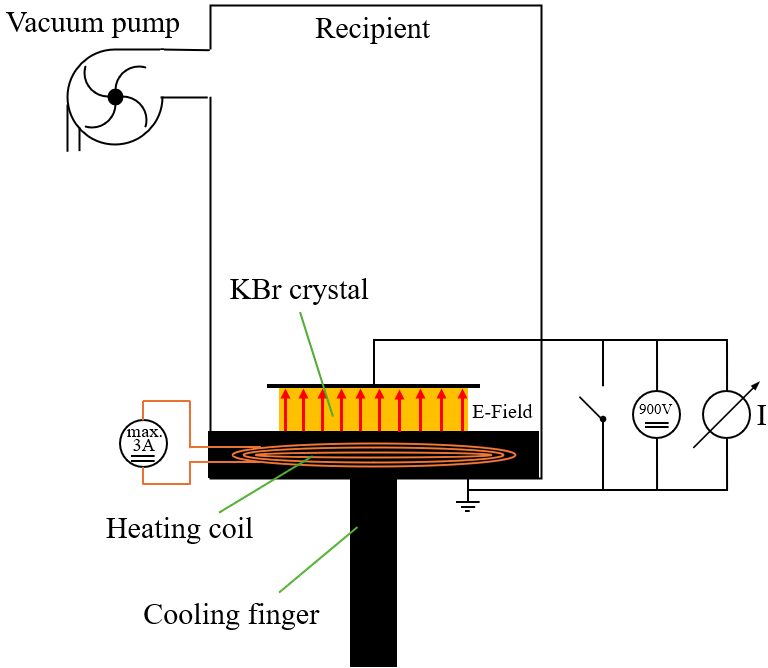
\includegraphics[height=6.5cm]{content/images/recipient.png}
        \caption{Sketch of the inside of the setup, design inspired by~\cite[2]{V48}.}
        \label{subfig:sketch}
    \end{subfigure}
    \hfill
    \begin{subfigure}{0.48\textwidth}
        \centering
        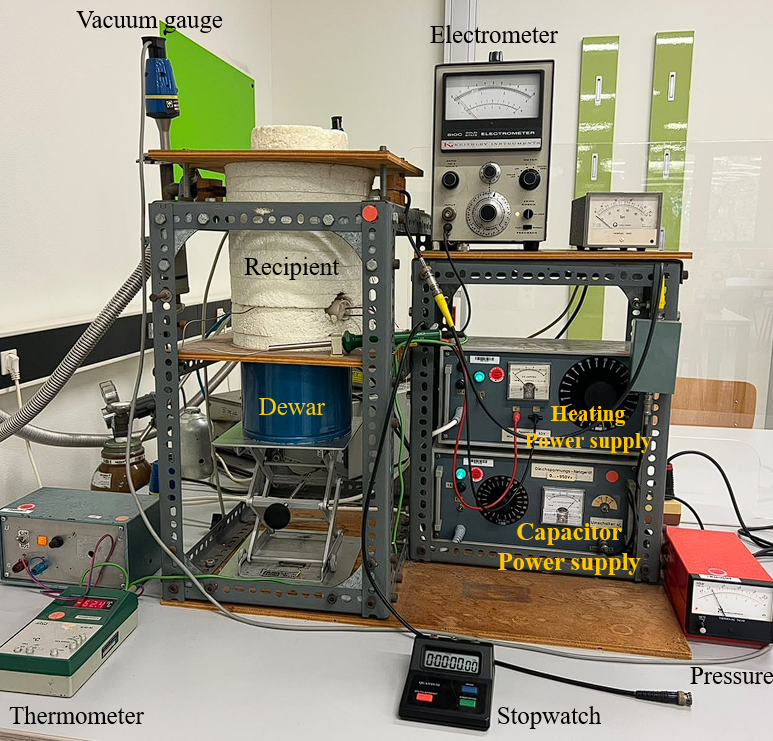
\includegraphics[height=6.5cm]{content/images/setup.png}
        \caption{Picture of the used setup.}
        \label{subfig:picture}
    \end{subfigure}
        \caption{Experimental setup, depicted as a photo and as a sketch.}
        \label{fig:setup}
\end{figure}
\FloatBarrier\noindent
To set the temperature of the crystal, the bottom of the recipient is connected to a copper cooling finger, that is inserted into a dewar filled with liquid nitrogen.
The submerged setup is shown in \autoref{subfig:picture}.
Heating the crystal is done with a heating coil inside the bottom of the recipient.
The temperature is shown on a digital thermostat, shown in the bottom left of \autoref{subfig:picture}.
The heating power is set by adjusting the heating current, with a maximum current of $I_{\max} = \qty{3}{\ampere}$.
\newline\noindent
For the measurement of the depolarisation current an electrometer is used.
It is set to picoamperes, for the depolarisation current as well as the noise are expected to be within this order of magnitude.
%
\subsection{Experimental procedure}
%
The experimented is conducted twice, with two different heating rates.
At first, a heating rate of $b_1 = \qty{2}{\kelvin\per\minute}$ is tried to be held.
For the second measurement, the heating rate is reduced to $b_2 = \qty{1.5}{\kelvin\per\minute}$.
Apart from this adaption, the experimental procedure is identical and is therefore only described once.
\newline\noindent
At first, the crystal has to be polarised. 
To reduce the polarisation time and to assure that most of the dipoles in the crystal are aligned, the crystal is heated to about $T = \qty{320}{\kelvin}$.
Then, the electric field is slowly ramped up to the maximum output voltage $U_{\max} = \qty{900}{\volt}$ of the power supply.
This state is then held for $t_{\mathrm{pol}} = \qty{900}{\second}$ to achieve nearly total polarisation.
The time is tracked with a digital stopwatch.
\newline\noindent
After the polarisation time has passed, the dewar is filled with liquid nitrogen and put under the recipient.
The cooling finger is inserted into the dewar until only a small gap between the wooden base plate of the recipient and the dewar is left. 
This setup is shown by \autoref{subfig:picture}.
The crystal is now cooled down to $T \approx \qty{180}{\degreeCelsius}$, with the E-field being still in place.
Because the liquid nitrogen vaporizes while cooling the crystal, the dewar has to be refilled to reach such low temperatures.
\newline\noindent
When the crystal has reached the desired temperature, the electric field is slowly ramped down and the capacitor is short-cuircuited for $t_{\mathrm{sc}} = \qty{300}{\second}$.
This corresponds to closing the switch in \autoref{subfig:sketch}.
In the experiment, it is done by reconnecting the BNC-cables of the two capacitor plates.
Whithin this time it is expected that the capacitor fully uncharges, so no noise current from remaining capacitor-induced current is measured.
\newline\noindent
To measure the depolarisation current, the upper capacitor plate is connected to the electrometer.
The heating current is then ramped up slowly.
With the digital stopwatch the heating rate is checked by comparing the temperature readings of the thermometer each minute.
Up to a temperature of $T_0 = \qty{210}{\kelvin}$ the heating is used to stabilize the heating rate.
The first data pair of temperature and depolarisation current is then taken at $T = T_0$.
The data is taken until the crystal temperature reaches $T_{\max} \approx \qty{330}{\kelvin}$.